% gruposlie.tex
%
% Copyright (C) 2022--2025 José A. Navarro Ramón <janr.devel@gmail.com>
% Licencia Creative Commons Recognition Share-alike.
% (CC-BY-SA)

\chapter{Grupos de Lie}
A bocajarro, definimos brevemente un grupo de Lie como un grupo que es una variedad
diferenciable, donde las operaciones del grupo son suaves o analíticas. Su estructura
es continua y \emph{suavemente deformable}. Más adelante se definirá de forma más
precisa.

Los grupos de Lie tienen mucha importancia en matemáticas y en física.
Aquí estamos interesados, principalmente, en su aplicación a la mecánica cuántica; en
particular, para comprender el concepto de spin en física de partículas, que en algunos
textos elementales se identifica incorrectamente con el giro de las partículas alrededor
de su eje.

\section{Rotaciones en el plano}
Para asimilar mejor el concepto de \emph{grupo de Lie}, empezamos analizando las rotaciones en $\symbb{R}^2$, olvidándonos por un momento de los grupos.
Las caracterizaremos de dos formas diferentes:
\begin{enumerate}
\item Mediante consideraciones trigonométricas.
\item Mediante una transformación que mantiene invariante la longitud.
\end{enumerate}

\subsection{Caracterización trigonométrica}
En la figura~\ref{fig:gli-x_axes} se representa un sistema de coordenadas cartesianas
rectangulares\footnotemark{} y un punto P cualquiera del espacio, con coordenadas
$(x_1,x_2)$, donde $\vvv{r}$ es el vector que indica su posición con respecto al origen.
\footnotetext{Denotamos los ejes de $\symbb{R}^2$ mediante $x_1$ y $x_2$,   igual que
  las coordenadas del punto. El lector no debería confundirlos, su interpretación se
  desprende del contexto.}
Las coordenadas de P con respecto a este sistema son
\begin{subequations}
  \begin{align}\label{eq:gli-coordxuno}
    x_1 &= r \cos(\alpha+\beta)\\
    \label{eq:gli-coordxdos}
    x_2 &= r \sin(\alpha+\beta)
  \end{align}
\end{subequations}
\begin{figure}[ht]
  \centering
  \begin{minipage}{0.40\linewidth}
    % Escala
    \def\scl{1}
    % Eje x
    \pgfmathsetmacro{\XMLONG}{0}
    \pgfmathsetmacro{\XPLONG}{3}
    % Eje y
    \pgfmathsetmacro{\YMLONG}{0}
    \pgfmathsetmacro{\YPLONG}{3}
    % Vector P
    \pgfmathsetmacro{\PMOD}{2.5}
    \pgfmathsetmacro{\PANG}{50}
    % Fondo
    \pgfmathsetmacro{\HORZ}{0.40}
    \pgfmathsetmacro{\VERT}{0.24}
    \pgfmathsetmacro{\MOD}{sqrt(\HORZ^2 + \VERT^2)}
    \pgfmathsetmacro{\ANGSD}{atan(\VERT / \HORZ)}
    \pgfmathsetmacro{\ANGII}{\ANGSD + 180.0}
    %
    \centering
    \begin{tikzpicture}[%
      scale=\scl,
      baseline,
      every node/.style={black,font=\small},
      eje/.style={->},
      vector/.style={-{Latex}, shorten >=1.2pt, line width=.8pt},
      dimmed/.style={lightgray, line width=.8pt, dotted},
      background/.style={
        line width=\bgborderwidth,
        draw=\bgbordercolor,
        fill=\bgcolor,
      },
      ]
      % Coordenadas
      \coordinate (O) at (0,0);
      \coordinate (xini) at (-\XMLONG cm,0);
      \coordinate (xfin) at (\XPLONG cm,0);
      \coordinate (yini) at (0,-\YMLONG cm);
      \coordinate (yfin) at (0,\YPLONG cm);
      \coordinate (P) at (\PANG:\PMOD cm);
      \path (O) -- coordinate (OPmidway) (P);
      % Ángulo alfa + beta
      \path (xfin) -- (O) -- (P)
%      pic [draw=black,fill=black!20,"\footnotesize $\alpha + \beta$",angle radius=6.3mm,
%      angle eccentricity=1.6,-{Latex[length=1.4mm,scale=.9,bend]}]
%      {angle = xfin--O--P};
      pic [draw=black,fill=black!20,"\footnotesize $\alpha + \beta$",angle radius=6.3mm,
      angle eccentricity=1.6]
      {angle = xfin--O--P};
      % Ejes
      \draw[eje] (xini) -- (xfin);
      \node[right, name=letraejex] at (xfin) {$x_1$};
      \coordinate (below) at ($(letraejex) - (0,1.0em)$);
      \draw[eje] (yini) -- (yfin);
      \node[above, name=letraejey] at (yfin) {$x_2$};
      \coordinate (left) at ($(letraejey) - (1.3em,0)$);
      % Vector de posición del punto P
      % \draw[black!70,-{Latex},shorten >=1.2pt] (O) -- (P);
      \draw[vector] (O) -- (P);
      \path (P |- xfin) coordinate (xm);
      \path (P -| yfin) coordinate (ym);
      \draw[dimmed] (P) -- (xm);
      \draw[dimmed] (P) -- (ym);
      \node[below] at (xm) {$x_1$};
      \node[left] at (ym) {$x_2$};
      \node[above=5pt] at (OPmidway) {$\vvv{r}$};
      % Punto
      \fill[fill=red,draw=black] (P) circle [radius=1.4pt];
      \node[above right] at (P) {$P$};
      % Origen
      \filldraw (O) circle [radius=.2pt];
      % Fondo amarillo
      \path (current bounding box.south west) ++(\ANGII:\MOD) coordinate (SW);
      \path (current bounding box.north east) ++(\ANGSD:\MOD) coordinate (NE);
      % \filldraw[draw=black, fill=red] (NE) circle[radius=1pt];
      \begin{scope}[on background layer]
        \draw[background] (SW) rectangle (NE);
      \end{scope}
    \end{tikzpicture}
    \caption{Ejes originales sin girar y punto P del plano, de coordenadas $(x_1,x_2)$.}
    \label{fig:gli-x_axes}
  \end{minipage}
  \hspace{1em}
  \begin{minipage}{0.45\linewidth}
    % Escala
    \def\scl{1}
    % Eje x
    \pgfmathsetmacro{\XMLONG}{0}
    \pgfmathsetmacro{\XPLONG}{3}
    % Eje y
    \pgfmathsetmacro{\YMLONG}{0}
    \pgfmathsetmacro{\YPLONG}{3}
    % Vector P
    \pgfmathsetmacro{\PMOD}{2.5}
    \pgfmathsetmacro{\PANG}{55}
    % Ángulo rotado
    \pgfmathsetmacro{\ANGROT}{20}
    \pgfmathsetmacro{\ANGROTPLUSNINETY}{\ANGROT + 90}
     % Fondo
    \pgfmathsetmacro{\HORZ}{0.25}
    \pgfmathsetmacro{\VERT}{0.35}
    \pgfmathsetmacro{\MOD}{sqrt(\HORZ^2 + \VERT^2)}
    \pgfmathsetmacro{\ANGSD}{atan(\VERT / \HORZ)}
    \pgfmathsetmacro{\ANGII}{\ANGSD + 180.0}
    % 
    \centering
    \begin{tikzpicture}[%
      scale=\scl,
      every node/.style={black,font=\small},
      ejerotado/.style={->},
      eje/.style={->, black!35},
      vector/.style={-{Latex}, shorten >=1.2pt, line width=.8pt},
      dimmed/.style={lightgray, line width=.8pt, dotted},
      background/.style={
        line width=\bgborderwidth,
        draw=\bgbordercolor,
        fill=\bgcolor,
      },      
      ]
      % Coordenadas
      \coordinate (O) at (0,0);
      \coordinate (xini) at (-\XMLONG cm,0);
      \coordinate (xfin) at (\XPLONG cm,0);
      \coordinate (yini) at (0,-\YMLONG cm);
      \coordinate (yfin) at (0,\YPLONG cm);
      \coordinate (x'ini) at (-\ANGROT:\XMLONG);
      \coordinate (x'fin) at (\ANGROT:\XPLONG);
      \coordinate (y'ini) at (-\ANGROTPLUSNINETY:\YMLONG);
      \coordinate (y'fin) at (\ANGROTPLUSNINETY:\YPLONG);
      \coordinate (P) at (\PANG:\PMOD cm);
      \path (O) -- coordinate (OPmidway) (P);
      % Ángulo alfa
      \path (xfin) -- (O) -- (x'fin) pic
      [draw=black,fill=green!30,"$\alpha$",angle radius=7mm,
      angle eccentricity=1.3,-{Latex[length=1.4mm,scale=.9,bend]}]
      {angle = xfin--O--x'fin};
      % Ángulo beta
      \path (x'fin) -- (O) -- (P) pic
      [draw=black!50!,fill=black!20,"$\beta$",angle radius=7mm, angle
      eccentricity=1.3] {angle = x'fin--O--P};
      % Ejes originales
      \draw[eje] (xini) -- (xfin);
      \node[right, name=letraejex, black!35] at (xfin) {$x_1$};
      \coordinate (below) at ($(letraejex) - (0,1.0em)$);
      \draw[eje] (yini) -- (yfin);
      \node[above, name=letraejey, black!35] at (yfin) {$x_2$};
      % Ejes rotados
      \draw[ejerotado] (O) -- (x'fin);
      % \path (O) -- node[pos=1.08,name=letraejexprima] {$x_1'$} (x'fin);
      \path (O) -- node[pos=1.08] {$x_1'$} (x'fin);
      \draw[ejerotado] (O) -- (y'fin);
      \path (O) -- node[pos=1.08] {$x_2'$} (y'fin);
      \path ($(O)!(P)!(x'fin)$) coordinate (x'm);
      \path ($(O)!(P)!(y'fin)$) coordinate (y'm);

      \draw[dimmed] (x'm) -- (P);
      \node[below, rotate=\ANGROT] at (x'm) {$x'_1$};
      \draw[dimmed] (y'm) -- (P);
      \node[left, rotate=\ANGROT] at (y'm) {$x'_2$};
      % Punto
      \draw[vector] (O) -- (P);
      \node[above=5pt] at (OPmidway) {$\vvv{r'}$};
      \fill[fill=red,draw=black] (P) circle [radius=1.4pt];
      \node[above right] at (P) {$P$};
      % Origen
      \filldraw (O) circle [radius=.2pt];
      % Fondo amarillo
      \path (current bounding box.south west) ++(\ANGII:\MOD) coordinate (SW);
      \path (current bounding box.north east) ++(\ANGSD:\MOD) coordinate (NE);
      % \filldraw[draw=black, fill=red] (NE) circle[radius=1pt];
      \begin{scope}[on background layer]
        \draw[background] (SW) rectangle (NE);
      \end{scope}      
    \end{tikzpicture}
    \caption{Ejes rotados un ángulo $\alpha$.
      Las coordenadas de P con respecto a estos nuevos ejes son $(x'_1,x'_2)$.}
    \label{fig:gli-rotated_axes}
  \end{minipage}
\end{figure}

En la figura~\ref{fig:gli-rotated_axes} llevamos a cabo una
\emph{rotación pasiva}\footnotemark{}, girando los ejes un ángulo $\alpha$ en sentido
positivo (antihorario).
Observe que no cambia la distancia, $r$, entre el punto y el origen, esto es, r'=r.
\footnotetext{En una rotación pasiva se gira el punto de vista (el sistema de
  referencia) y no el punto.}
Las coordenadas del punto P con respecto del sistema girado son
\begin{subequations}
  \begin{align}\label{eq:gli-coordxprimauno}
    x_1' &= r \cos\beta\\
    \label{eq:gli-coordxprimados}
    x_2' &= r \sin\beta
  \end{align}
\end{subequations}

Desarrollamos~\eqref{eq:gli-coordxuno} y~\eqref{eq:gli-coordxdos} y
utilizamos~\eqref{eq:gli-coordxprimauno} y~\eqref{eq:gli-coordxprimados}
\begin{align*}
  x_1 &= r \cos\alpha \cos\beta - r \sin\alpha \sin\beta
        = \cos\alpha\,(r\cos\beta) - \sin\alpha\,(r\sin\beta)\\
        &= \cos\alpha\cdot x_1' - \sin\alpha \cdot x_2'\\
  x_2 &= r \sin\alpha \cos\beta + r \cos\alpha \sin\beta
        = \sin\alpha\,(r \cos\beta) + \cos\alpha\,(r \sin\beta)\\
        &= \sin\alpha \cdot x_1' + \cos\alpha \cdot x_2'
\end{align*}

Estas dos últimas expresiones se pueden representar en forma matricial
\[
  \begin{pmatrix}
    x_1 \\[0.4ex] x_2
  \end{pmatrix}
  =
  \begin{pmatrix}
    \cos\alpha & -\sin\alpha\\[0.3ex] \sin\alpha & \cos\alpha
  \end{pmatrix}
  \begin{pmatrix}
    x_1' \\[0.3ex] x_2'
  \end{pmatrix}
\]

Llamando $\mmm{M}$ a la matriz de la transformación, $\vvv{x}$ y $\vvv{x'}$
a los vectores que representan las coordenadas del punto sin rotar y rotado,
respectivamente, la ecuación anterior queda
\begin{equation}\label{eq:gli-rotpasiva_inversa_vectores}
  \vvv{x} = \mmm{M} \vvv{x'}
\end{equation}

Estamos interesados en la transformación inversa, esto es,
queremos hallar las nuevas coordenadas de P respecto al sistema
girado si conocemos las que tiene el punto en el sistema original,
$\vvv{x'} = \mmm{R} \vvv{x}$, donde $\mmm{R}$ será la matriz de rotación
pasiva.
Para resolver la ecuación anterior, hay que multiplicar por la
izquierda\footnotemark{} la inversa de la matriz $\mmm{M}$ en la
ecuación~\eqref{eq:gli-rotpasiva_inversa_vectores}
\footnotetext{Se multiplica por la izquierda porque las matrices cuadradas
  junto con el producto de matrices, forman un grupo no conmutativo.}
\[
  \mmm{M}^{-1}\vvv{x} = \mmm{M}^{-1}\mmm{M}\vvv{x'}
\]
\[
  \mmm{M}^{-1}\vvv{x} = \mmm{I}\vvv{x'}
\]
\[
  \vvv{x'} = \mmm{M}^{-1}\vvv{x}
\]
Y como
\[
  \vvv{x'} = \mmm{R}\vvv{x}
\]
Se deduce que la matriz de rotación pasiva es la inversa de $\mmm{M}$
\[
  \mmm{R} = \mmm{M}^{-1}
\]

Antes de nada, debemos comprobar que la matriz $\mmm{M}$ tiene inversa; para ello su
determinante no puede ser nulo\footnotemark{}.
\footnotetext{Una matriz con determinante cero se llama \emph{matriz singular}
  y no tiene inversa.}

Calculamos el determinante y comprobamos que no es nulo, por lo que tiene inversa
\begin{equation}\label{eq:gli-determinante_M}
  \det \mmm{M}
  =
  \begin{vmatrix}
    \cos\alpha & -\sin\alpha \\ \sin\alpha & \cos\alpha
  \end{vmatrix}
  = \cos^2\alpha + \sin^2\alpha = 1
\end{equation}

La inversa de una matriz es igual a la adjunta de la traspuesta dividida entre su
determinante
\[
  \mmm{M}^{-1} = \dfrac{1}{\det(\mmm{M})}\,\text{adj} \left(\mmm{M}^\trasp\right)
\]

 Nuestra matriz $\mmm{M}$ es
\[
  \mmm{M}
  =
  \begin{pmatrix}
    \cos\alpha & -\sin\alpha\\ \sin\alpha & \cos\alpha
  \end{pmatrix}
\]

Primero hallamos la traspuesta, que se obtiene al intercambiar filas por columnas
\[
  \mmm{M}^\trasp
  =
  \begin{pmatrix}
    B_{11} & B_{12}\\ B_{21} & B_{22}
  \end{pmatrix}
  =
  \begin{pmatrix}
    \cos\alpha & \sin\alpha\\ -\sin\alpha & \cos\alpha
  \end{pmatrix}
\]

Vamos a obtener la adjunta (o de los cofactores) de la traspuesta, razonando elemento
por elemento --ya que no se hace muy pesado, por tener solo cuatro elementos--
\[
  \text{adj}\left(\mmm{M^\trasp}\right)
    = \begin{pmatrix}
        A_{11} & A_{12} \\ A_{21} & A_{22}
      \end{pmatrix}
\]

El cofactor, $A_{ij}$, de cada elemento $B_{ij}$ se obtiene multiplicando $(-1)^{\,i+j}$
por el menor complementario de $B_{ij}$.
El menor complementario es el determinante que queda al eliminar la fila $i$ y la $j$ de
la matriz.

Calculamos el cofactor de cada uno de los elementos de la matriz traspuesta. El elemento
lo indicamos con letras en rojo. En este caso, debido a que la matriz es $2\times 2$, el
menor complementario es un determinante formado por un único elemento, que no se marca
con fondo rojo
\begin{align*}
  A_{11}
  &= \text{cof}\,(B_{11})
    = (-1)^{1+1}\,\text{det}
    \begin{pNiceArray}{rr}
      \textcolor{red!80!black}{\cos\alpha} & \textcolor{black!70}{\sin\alpha}\\
      \textcolor{black!70}{-\sin\alpha} & \cos\,\alpha
      \CodeAfter
      \tikz \draw[red,line width=10pt,opacity=0.15] (1.5-|1) -- (1.5-|last);
      \tikz \draw[red,line width=30pt,opacity=0.15] (1.5|-1) -- (1.5|-last);
    \end{pNiceArray}
    = \text{det}\,(\cos\alpha)
    = \cos\alpha\\
  A_{12}
  &= \text{cof}\,(B_{12})
    = (-1)^{1+2}\,\text{det}
    \begin{pNiceArray}{rr}
      \textcolor{black!70}{\cos\alpha} & \textcolor{red!80!black}{\sin\alpha}\\
      \textcolor{black}{-\sin\alpha} & \textcolor{black!70}{\cos\alpha}
      \CodeAfter
      \tikz \draw[red,line width=10pt,opacity=0.15] (1.5-|1) -- (1.5-|last);
      \tikz \draw[red,line width=30pt,opacity=0.15] (2.5|-1) -- (2.5|-last);
    \end{pNiceArray}
    = - \text{det}\,(-\sin\alpha)
    = \sin\alpha\\
  A_{21}
  &= \text{cof}\,(B_{21})
    = (-1)^{2+1}\,\text{det}
    \begin{pNiceMatrix}
      \textcolor{black!70}{\cos\alpha} & \textcolor{black}{\sin\alpha}\\
      \textcolor{red!80!black}{-\sin\alpha} & \textcolor{black!70}{\cos\alpha}
      \CodeAfter
      \tikz \draw[red,line width=10pt,opacity=0.15] (2.5-|1) -- (2.5-|last);
      \tikz \draw[red,line width=30pt,opacity=0.15] (1.5|-1) -- (1.5|-last);
    \end{pNiceMatrix}
    = -\text{det}\,(\sin\alpha)
    = -\sin\alpha\\
  A_{22}
  &= \text{cof}\,(B_{22})
    = (-1)^{2+2}\,\text{det}
    \begin{pNiceMatrix}
      \textcolor{black}{\cos\alpha} & \textcolor{black!70}{\sin\alpha}\\
      \textcolor{black!70}{-\sin\alpha} & \textcolor{red!80!black}{\cos\alpha}
      \CodeAfter
      \tikz \draw[red,line width=10pt,opacity=0.15] (2.5-|1) -- (2.5-|last);
      \tikz \draw[red,line width=30pt,opacity=0.15] (2.5|-1) -- (2.5|-last);
    \end{pNiceMatrix}
    = \det\,(\cos\alpha)
    = \cos\alpha
\end{align*}

La matriz de cofactores de la traspuesta resulta
\[
  \text{adj} (\mmm{M}^\trasp)
  =
  \begin{pmatrix}
    A_{11} & A_{12}\\ A_{21} & A_{22}
  \end{pmatrix}
  =
  \begin{pmatrix}
    \cos\alpha & \sin\alpha\\
    -\sin\alpha & \cos\alpha
  \end{pmatrix}
\]
Teniendo en cuenta que el determinante de la matriz valía la unidad, ver
\eqref{eq:gli-determinante_M}, la matriz inversa es
\[
  \mmm{M}^{-1}
  =
  \dfrac{1}{\det(\mmm{M})}\,
  \begin{pmatrix}
    \cos\alpha & \sin\alpha\\
    -\sin\alpha & \cos\alpha
  \end{pmatrix}
  =
  \dfrac{1}{1}\,
  \begin{pmatrix}
    \cos\alpha & \sin\alpha\\
    -\sin\alpha & \cos\alpha
  \end{pmatrix}
  =
  \begin{pmatrix}
    \cos\alpha & \sin\alpha\\
    -\sin\alpha & \cos\alpha
  \end{pmatrix}
\]

Es instructivo señalar que, en este caso, la inversa es igual a la traspuesta y resulta
ser la matriz de rotación pasiva $\mmm{R}$ que buscamos
\begin{equation}
  \label{eq:gli-matriz_rotacion_2x2}
  \mmm{R}
  =
  \mmm{M}^{-1}
  =
  \mmm{M}^\trasp
  =
  \begin{pmatrix}
    \cos\alpha & \sin\alpha\\
    -\sin\alpha & \cos\alpha
  \end{pmatrix}
\end{equation}

Las nuevas coordenadas, $\vvv{x'}$, se obtienen aplicando la matriz de rotación a las
del sistema sin girar, $\vvv{x}$
\[
  \vvv{x'} = \mmm{R} \vvv{x}
\]

\[
  \begin{pmatrix}
    x'_1\\[0.4ex]x'_2
  \end{pmatrix}
  =
  \begin{pmatrix}
    \cos\alpha & \sin\alpha\\
    -\sin\alpha & \cos\alpha
  \end{pmatrix}
  \,
  \begin{pmatrix}
    x_1 \\ x_2
  \end{pmatrix}
\]

\subsubsection{Criterio de la suma de Einstein}
Abandonamos por un instante nuestro guión para explicar la notación de Einstein.
Supongamos que queremos calcular las coordenadas $\vvv{x'}$ mediante el producto
matricial
\[
  \begin{pmatrix}
    x'_1\\[0.4ex] x'_2
  \end{pmatrix}
  =
  \begin{pmatrix}
    R_{11} & R_{12}\\
    R_{21} & R_{22}
  \end{pmatrix}
  \,
  \begin{pmatrix}
    x_1 \\ x_2
  \end{pmatrix}  
\]
\begin{align*}
  x'_1 &= R_{11} x_1 + R_{12} x_2\\
  x'_2 &= R_{21} x_1 + R_{22} x_2
\end{align*}

Obtenemos que el elemento $x'_i$ de $\vvv{x'}$ se calcula mediante un sumatorio
\begin{equation}\label{eq:gli-sumatorio}
  x'_i = \sum_{j=1}^2 R_{ij} x_j
  \hspace*{3em}
  (i = 1,2)
\end{equation}

Observamos que el índice de la suma es el que se repite (el $j$ en este caso),
por lo que podemos eliminar el símbolo del sumatorio siempre que
consideremos que hay que aplicarlo cuando aparezcan índices repetidos
\begin{equation}\label{eq:gli-criteriosumaeinstein}
  x'_i = R_{ij} x_j
  \hspace*{3em}
  (i = 1,2)
\end{equation}

Cuando se utiliza el criterio de la suma de Einstein, las expresiones son más
fáciles de escribir; en nuestro caso, las~\eqref{eq:gli-criteriosumaeinstein}
son totalmente equivalentes a las~\eqref{eq:gli-sumatorio}.

\subsection[Mediante transformación que deja invariante la longitud]
{Caracterización por medio de una transformación que deja invariante la
  longitud}\label{invariante_longitud}
Ahora nos olvidaremos de la trigonometría y deduciremos las características de la matriz
de rotación $\mmm{R}$ de una manera más sofisticada.

Cuando se realiza una rotación, las distancias se deben conservar.
En nuestro ejemplo de la figura~\ref{fig:gli-rotated_axes}, la distancia $r = |\vvv{r}|$
del origen al punto es la misma en cualquiera de los sistemas de coordenadas, el
original y el girado.

Abordaremos este apartado de dos formas; en la primera, desarrollaremos los cálculos con
todo detalle y, en la segunda, seguiremos un razonamiento aún más sofisticado y potente.

\subsubsection{Desarrollo con gran detalle}
Llamemos $s$ a la distancia que se conserva, por ejemplo la distancia entre el punto P y
el origen en la figura~\eqref{fig:gli-rotated_axes}
\[
  s = \sqrt{x'^2_1 + x'^2_2}
  = \sqrt{x^2_1 + x^2_2}
\]

La invariancia de distancias se expresa más cómodamente sin raíces cuadradas
\begin{equation}
  \label{eq:gli-invariancia_dist}
  s^2 = x'^2_1 + x'^2_2
  = x^2_1 + x^2_2
\end{equation}

Además sabemos que las nuevas coordenadas se obtendrán a partir de las antiguas a través
de una matriz de rotación
\[
  \begin{pmatrix}
    x'_1 \\[0.4ex] x'_2
  \end{pmatrix}
  =
  \begin{pmatrix}
    R_{11} & R_{12}\\
    R_{21} & R_{22}
  \end{pmatrix}
  \,
  \begin{pmatrix}
    x_1 \\ x_2
  \end{pmatrix}
\]

Desarrollando, obtenemos las nuevas $(x'_1,x'_2)$ a partir de las originales, $(x_1,x_2)$
\begin{align*}
  x'_1 &= R_{11} x_1 + R_{12} x_2\\
  x'_2 &= R_{21} x_1 + R_{22} x_2
\end{align*}

Obligamos a que se cumpla~\eqref{eq:gli-invariancia_dist}
\begin{align*}
  s^2 &= x'^2_1 + x'^2_2\\
      &= (R_{11} x_1 + R_{12} x_2)^2 + (R_{21} x_1 + R_{22} x_2)^2\\
      &= R^2_{11} x^2_1 + R^2_{12} x^2_2 + 2 R_{11} R_{12} x_1 x_2
        + R^2_{21} x^2_1 + R^2_{22} x^2_2 + 2 R_{21} R_{22} x_1 x_2\\
      &= (R^2_{11} + R^2_{21}) x^2_1 + (R^2_{12} + R^2_{22}) x^2_2
        + 2 (R_{11} R_{12} + R_{21} R_{22}) x_1 x_2\\
      &= x^2_1 + x^2_2
\end{align*}

Identificando coeficientes, los elementos de la matriz de rotación deben cumplir
\begin{align*}
  &R^2_{11} + R^2_{21} = 1\\
  &R^2_{22} + R^2_{12} = 1\\
  & R_{11} R_{12} + R_{21} R_{22} = 0
\end{align*}

No hemos obtenido el valor de la matriz de rotación en dos dimensiones como en la
sección anterior, pero hemos llegado a unas igualdades que deben cumplir sus elementos.

Multiplicamos la traspuesta de la matriz por la matriz e imponemos las relaciones que
deben cumplir los elementos de la matriz de rotación
\begin{align*}
  \mmm{R}^\trasp \mmm{R}
  &=
  \begin{pmatrix}
    R_{11} &  R_{21}\\
    R_{12} & R_{22}
  \end{pmatrix}
  \,
  \begin{pmatrix}
    R_{11} &  R_{12}\\
    R_{21} & R_{22}
  \end{pmatrix}
  =
  \begin{pmatrix}
    R^2_{11} + R^2_{21} & R_{11} R_{12} + R_{21} R_{22}\\
    R_{12} R_{11} + R_{22} R_{21} & R^2_{12} + R^2_{22}
  \end{pmatrix}\\
  &=
    \begin{pmatrix}
    1 &  0 \\
    0 & 1
  \end{pmatrix}
\end{align*}

Hemos demostrado que al imponer la condición de que para que se conserven las distancias
en una rotación, la matriz inversa de la rotación debe ser igual a la traspuesta,
$\mmm{R}^{-1} = \mmm{R}^\trasp$
\[
  \mathbf{R}^\trasp \mathbf{R} = \mathbf{I}
\]

\subsubsection{Desarrollo más sofisticado}
Vamos a llegar a la misma conclusión pero de una forma más sofisticada y, de hecho, no
especificaremos la dimensión del espacio donde se produce la rotación; recordemos que en
los desarrollos anteriores siempre hemos supuesto que la rotación se producía en el
plano $\symbb{R}^2$, de dimensión 2.

Primero hay que introducir una expresión matricial para el producto escalar de un vector
por sí mismo y para ello nos viene bien suponer, momentáneamente, el espacio de
dimensión dos.
El producto escalar del vector columna $\vvv{x}$ por sí mismo es un escalar no negativo
que llamaremos $s^2$ y se calcula multiplicando la traspuesta del vector por él mismo
\[
  |\vvv{x}|^2 = \vvv{x}\cdot\vvv{x}
  = \vvv{x}^\trasp \vvv{x}
  =
  \begin{pmatrix}
    x_1 \\ x_2
  \end{pmatrix}^\trasp
  \,
  \begin{pmatrix}
    x_1 \\ x_2
  \end{pmatrix}
  =
  \begin{pmatrix}
    x_1 & x_2
  \end{pmatrix}
  \,
  \begin{pmatrix}
    x_1 \\ x_2
  \end{pmatrix}
  = x^2_1 + x^2_2 = s^2
\]

Demostraremos, sin tener en cuenta la dimensión del espacio, que la inversa de la matriz
de rotación es la traspuesta.

Sabemos que la cantidad invariante es $s²$, que se puede expresar en función de las
coordenadas rotadas y de las originales
\begin{equation}\label{eq:gli-s2xprime}
  (\vvv{x'})^\trasp \vvv{x'} = \vvv{x}^\trasp \vvv{x} = s^2
\end{equation}

Además, sabemos que estas coordenadas $\vvv{x'}$ se obtienen aplicando la matriz de
rotación a las coordenadas sin rotar
\[
  \vvv{x'} = \mmm{R} \vvv{x}
\]

Su traspuesta será
\[
  (\vvv{x'})^\trasp = (\mmm{R} \vvv{x})^\trasp = \vvv{x}^\trasp \mmm{R}^\trasp
\]

Sustituimos esta expresión en la ecuación~\eqref{eq:gli-s2xprime}
\[
  (\vvv{x'})^\trasp \vvv{x'}
  = \vvv{x}^\trasp \mmm{R}^\trasp \mmm{R} \vvv{x}
  = \vvv{x}^\trasp \vvv{x} = s^2
\]

Se desprende de la ecuación anterior que
\begin{equation}\label{eq:gli-R_ortogonal}
  \mmm{R}^\trasp \mmm{R} = \mmm{I}
\end{equation}

Recalcamos que hemos llegado a esta conclusión sin presuponer la dimensión del espacio,
por lo que hemos demostrado que se debe cumplir sea cual sea esta.

¿Qué podemos decir del determinante de $\mmm{R}$?
\[
  \det(\mmm{R}^\trasp \mmm{R})
  =
  \det\left(\mmm{I}\right)
\]
\[
  \det\left(\mmm{R}^\trasp\right)\,\det\left(\mmm{R}\right)
  = 1
\]
\[
  \det\left(\mmm{R}\right)\,\det\left(\mmm{R}\right)
  = 1
\]
\[
 \left[\det(\mmm{R})\right]^2 = 1
\]

Así que
\[
  \det(\mmm{R}) = \pm 1
\]

El valor $-1$ corresponde a una reflexión y no a una rotación, por lo que hemos de
descartar este valor, quedando
\begin{equation}\label{eq:gli-detRuno}
  \det(\mmm{R}) = 1
\end{equation}


\section{El grupo de rotaciones}
Vamos puntualizar algunos detalles acerca de la matriz de rotación:
\begin{itemize}
\item La matriz de rotación depende de la dimensión del espacio; cuando vale 2, es
  \begin{equation}\label{eq:gli-rotacion2x2}
    \mmm{R}(\alpha)
    =
    \begin{pmatrix}
      \cos\alpha & \sin\alpha\\
      -\sin\alpha & \cos\alpha
    \end{pmatrix}
  \end{equation}
  
  Aunque esta matriz la dedujimos anteriormente a partir de consideraciones
  trigonométricas, la volveremos a obtener a partir del concepto
  \emph{generador de una rotación}, que se introducirá en la sección siguiente
  \ref{sec:defgrupolie}.
  
\item Las matrices de rotación dependen de un parámetro (el ángulo), que es una variable
  continua, $\mmm{R} (\alpha)$.

\item Las matrices que cumplen que su inversa es igual a la
  traspuesta~\eqref{eq:gli-R_ortogonal}, como ocurre con este tipo de matrices, se dice
  que son \emph{ortogonales}. Además, para que se trate de rotaciones, tienen que tener
  un determinante igual a $+1$, ver la ecuación~\eqref{eq:gli-detRuno}. Estas matrices
  suelen presentarse en las transformaciones entre bases de espacios vectoriales.

\item El conjunto de las matrices de rotación, junto con el producto ordinario de
  matrices, forma un grupo, $G$, infinito y continuo
  \[
    G = \{ \mmm{R}\,|\,\mmm{R}^\trasp \mmm{R} = \mmm{I}, \det \mmm{R} = 1 \}
  \]

  Para demostrar que es un grupo, debemos probar que el producto cumple las tres
  propiedades:
  \begin{enumerate}
  \item Propiedad asociativa: Sabemos que el producto de matrices cuadradas cumple la
    propiedad asociativa, por lo que el producto de matrices de rotación, que forman un
    subconjunto de aquellas, también la cumple.
  \item Existencia de elemento identidad: El elemento identidad en el producto de
    matrices es la matriz unitaria. Demostraremos que la matriz unitaria es un elemento
    del conjunto de matrices de rotación. Esto se demuestra haciendo $\alpha = 0$, por
    ejemplo, en la matriz de rotación en dos dimensiones de la ecuación
    \eqref{eq:gli-rotacion2x2}
    \[
      \mmm{R}(0) =
      \begin{pmatrix}
        \cos 0 & \sin 0\\
        -\sin 0 & \cos 0
      \end{pmatrix}
      =
      \begin{pmatrix}
        1 & 0 \\
        0 & 1
      \end{pmatrix}
      = \mmm{I}
    \]
  \item Existencia de elemento inverso: Como el determinante de la matriz de rotación no
    es nulo, existe la matriz de rotación inversa.
  \end{enumerate}
\end{itemize}

\section{Definición de Grupo de Lie}\label{sec:defgrupolie}
El grupo de rotaciones es un conjunto infinito porque  $\mmm{R}(\alpha)$ tiene un
elemento por cada valor del ángulo $\alpha$
\[
  0 \leq \alpha < 2\,\pi
\]
y hay infinitos números reales $\alpha$ entre $0$ y $2\pi$.

Además es un conjunto continuo, porque $\alpha$ varía continuamente, esto es, no hay
discontinuidades entre dos valores de $\alpha$, siempre podremos encontrar infinitos
números reales entre dos cualesquiera por cercanos que parezcan.

Todo grupo infinito y continuo se llama \emph{grupo de Lie}. Una definición más completa
sería:
\begin{quote}
  \emph{Un grupo de matrices de Lie --abreviadamente grupo de Lie-- es un subgrupo
    continuo de las matrices cuadradas $N\times N$ no singulares sobre un campo $K$
    --que suele ser $\symbb{R}$ o $\symbb{C}$--.}
\end{quote}

\emph{Continuo} es una forma de expresar que un grupo de Lie es una \emph{variedad}
(\emph{manifold} en inglés).
Esta propiedad permite que se pueda hablar de una función $\mmm{R}$, que asocia a cada
número real $\alpha$ una matriz cuadrada no singular
$\mmm{R}(\alpha)$
\begin{center}
  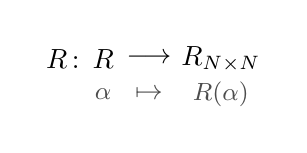
\begin{tikzpicture}[%
      baseline,
      fila2/.style={black!70,font=\small},
    ]
    \matrix (mymatrix)[row sep=-3pt, column sep=-2pt]
    {
      \node{$\mmm{R}$\,:}; & \node{$\symbb{R}$}; & \node{$\longrightarrow$}; &
      [-1pt]\node{$\mmm{R}_{N\times N}$};\\
      & \node[fila2]{$\alpha$}; & \node[black!70]{$\mapsto$}; &
      \node[fila2]{$\mmm{R}(\alpha)$};\\
  };
\end{tikzpicture}
\end{center}

Un ejemplo de grupo de Lie es el que se representa como O(N), que es el grupo de las
matrices ortogonales $N\times N$; esto es, el grupo de matrices $\mmm{A}$ de componentes
reales que cumplen
\[
  \mmm{A}^{\trasp} \mmm{A} = \mmm{I}
\]

La igualdad anterior implica que
\[
  \det(\mmm{A}) = \pm 1
\]
y es válida para el grupo de rotaciones con $\det(\mmm{A}) = +1$ y para el de
reflexiones, con $\det(\mmm{A}) = -1$, en un espacio de dimensión $N$.

\[
  O(2)
  = \{ \mmm{R}(\alpha)\ |\ \mmm{R}\text{ es matriz real } 2\times 2, \mmm{R}^\trasp
  \mmm{R} = \mmm{I},\ \det(\mmm{R}) = \pm 1\}
\]


En estas transformaciones (rotaciones y reflexiones) se conserva el módulo de los
vectores del espacio
\[
  (\vvv{x}')^{2}
  = (\mmm{A}\vvv{x})^{2}
  = (\mmm{A}\vvv{x})^{\trasp} (\mmm{A}\vvv{x})
  = \vvv{x}^{\trasp} \mmm{A}^{\trasp} \mmm{A} \vvv{x}
  = \vvv{x}^{\trasp} \mmm{I} \vvv{x}
  = \vvv{x}^{\trasp} \vvv{x}
  = \vvv{x}^{2}
\]

El grupo SO(N) es el subgrupo de matrices de O(N) con determinante unidad, esto es, el
grupo de rotaciones --sin incluir las reflexiones--.

\subsubsection{SO(2)}
El grupo de rotaciones de dimensión 2 se suele representar como SO(2):
\begin{itemize}
\item La $S$ significa que las matrices son especiales
  \[
    \det(\mmm{R}) = 1
  \]
\item La $O$, que las matrices son ortogonales
  \[
    \mmm{R}^\trasp \mmm{R} = \mmm{I}
  \]
\item El $2$ hace referencia a que se trata de un grupo de matrices $2\times 2$.
\end{itemize}
Por ejemplo, el conjunto que forma el grupo de rotaciones de dimensión 2 se puede definir
\[
  SO(2)
  = \{ \mmm{R}(\alpha)\ |\ \mmm{R}\text{ es matriz real } 2\times 2, \mmm{R}^\trasp
  \mmm{R} = \mmm{I},\ \det(\mmm{R}) = 1\}
\]
que es el grupo de matrices ortogonales $2\times 2$, que describen la rotación en el
plano real y forman un grupo de Lie.

\subsection{Matriz de rotación general}\label{sec:matriz_rotacion_general}
Tenemos las siguientes propiedades de la matriz de rotación,
ecuaciones~\eqref{eq:gli-R_ortogonal} y~\eqref{eq:gli-detRuno}
\begin{align*}
  \mmm{R}^\trasp \mmm{R} &= \mmm{I}\\
  \det(\mmm{R}) &= 1
\end{align*}
y hemos obtenido una expresión concreta cuando la dimensión es 2,
ver~\eqref{eq:gli-rotacion2x2}
\[
  \mmm{R}(\alpha)
  = \begin{pmatrix}
    \cos\alpha & \sin\alpha\\
    -\sin\alpha & \cos\alpha
    \end{pmatrix}
\]

Nos proponemos hallar la expresión general para la matriz de rotación,
independientemente de la dimensión del espacio en el que se realiza la transformación
(simplificando bastante la notación).

Supongamos que queremos rotar un sistema un ángulo finito $0 \leq \alpha < 2\pi$.
Sabemos que rotar un ángulo $\alpha$ equivale a rotar $N$ veces el ángulo $\alpha / N$.
En particular, estamos interesados en valores de $N$ muy grandes, que tienden a
infinito, es decir, valores para los que $\varepsilon=\alpha/N$ sea una cantidad
infinitesimal
\[
  \alpha = N\,\dfrac{\alpha}{N} = N \varepsilon
\]

Si un parámetro $\varepsilon$ es infinitesimal, en primera aproximación, se considera
que su cuadrado es despreciable ($\varepsilon^2\approx 0$).

Una rotación infinitesimal cambia algo el objeto rotado, pero muy poco, de manera que
casi lo deja igual. Esto se puede representar matemáticamente
\[
  \mmm{R}(\varepsilon) = \mmm{R}\left(\dfrac{\alpha}{N}\right) = \mmm{I} + \mmm{A}
\]
donde $\mmm{A}$ es una matriz infinitesimal.

La rotación finita sería el resultado de aplicar sucesivamente un número $N$ (que tiende
a infinito) de rotaciones, de manera que hay que multiplicar $\mmm{R}(\varepsilon)$ por
sí misma, $N$ veces
\[
  \mmm{R} (\alpha)
  = \underbrace{%
    \mmm{R}(\varepsilon) \mmm{R}(\varepsilon) \cdots \mmm{R}(\varepsilon)
    }_{N\text{ veces}}
  = \mmm{R}(\varepsilon)^N = (\mmm{I} + \mmm{A})^N
\]

Analicemos cómo debería ser la matriz infinitesimal $\mmm{A}$.
La matriz de rotación infinitesimal $\mmm{R}(\varepsilon) = \mmm{I} + \mmm{A}$,
por ser matriz de rotación, debe ser ortogonal
\[
  \mmm{R}^\trasp \mmm{R} = \mmm{I}
\]
\[
  (\mmm{I} + \mmm{A})^\trasp \, (\mmm{I} + \mmm{A}) = \mmm{I}
\]
\[
  (\mmm{I}^\trasp + \mmm{A}^\trasp)\, (\mmm{I} + \mmm{A}) = \mmm{I}
\]
\[
  (\mmm{I} + \mmm{A}^\trasp)\, (\mmm{I} + \mmm{A}) = \mmm{I}
\]
\[
  \mmm{I} \mmm{I}
  + \mmm{I} \mmm{A}
  + \mmm{A}^\trasp \mmm{I}
  + \mmm{A}^\trasp \mmm{A}
  = \mmm{I}
\]
\[
  \mmm{I} + \mmm{A} + \mmm{A}^\trasp + \symcal{O}\left(A^2\right) = \mmm{I}
\]

Nótese que $\mmm{A}^\trasp \mmm{A}$ es despreciable porque $\mmm{A}$ es infinitesimal.
La expresión~\eqref{eq:gli-A_antisimetrica} que se obtiene, define a la matriz \mmm{A}
como antisimétrica, $\mmm{A}^\trasp = -\mmm{A}$
\begin{equation}\label{eq:gli-A_antisimetrica}
  \mmm{A} + \mmm{A}^\trasp = 0
\end{equation}

Los elementos de las matrices antisimétricas, como $\mmm{A}$, cumplen $A_{ij} = -A_{ji}$.
Nótese que los elementos diagonales de las matrices antisimétricas deben ser cero para
que se cumpla $A_{ii} = -A_{ii}$.

Hay dos opciones para $\mmm{A}$, reflejadas en~\eqref{eq:gli-opcionesA}, cada una es la
opuesta de la otra.
En principio cualquiera sería válida.
La clave reside en el significado que le demos al ángulo de rotación $\varepsilon$.
Podría definirse como el ángulo que giran los ejes o el que giran los vectores; cada uno
de los ángulos es opuesto del otro, de ahí que las dos matrices posibles sean inversas
\begin{equation}\label{eq:gli-opcionesA}
  \mmm{A}
  =
  \begin{pmatrix}
    0 & \varepsilon\\
    -\varepsilon & 0
  \end{pmatrix}
  \hspace{1em}
  \text{o}
  \hspace{1em}
  \mmm{A}
  =
  \begin{pmatrix}
    0 & -\varepsilon\\
    \varepsilon & 0
  \end{pmatrix}
\end{equation}

Sólo tenemos un grado de libertad, $\varepsilon$.
De acuerdo con nuestro convenio de rotación pasiva (giro de los ejes de coordenadas),
definimos $\varepsilon$ como \emph{el ángulo que giran los ejes de coordenadas},
teniendo en cuenta que el sentido positivo es el antihorario.
¿Cómo podemos saber cuál de las dos matrices anteriores es la que se corresponde con
nuestro convenio?

Para dilucidarlo, hacemos girar infinitesimalmente los ejes en sentido positivo, por lo
tanto los vectores aparentarán girar en sentido negativo, tal y como se aprecia en la
figura~\ref{fig:gli-girovector}.
Ahora construimos las transformaciones que se obtienen y vemos que la coordenada $x$
aumenta ligeramente, de ahí la suma en la expresión~\eqref{eq:gli-giro_incx}; en cambio,
la coordenada $y$ disminuye ligeramente, y la ecuación~\eqref{eq:gli-giro_incy}
representa esta transformación
\begin{subequations}\label{eq:gli-giro_incxy}
  \begin{align}
    \label{eq:gli-giro_incx}
    x' &= x + \varepsilon y \\
    \label{eq:gli-giro_incy}
    y' &= y - \varepsilon x
  \end{align}
\end{subequations}

Podemos resumir de forma matricial las ecuaciones~\eqref{eq:gli-giro_incxy} anteriores
\begin{equation}\label{eq:gli-giro_incxy_matricial}
  \begin{pmatrix}
    x' \\ y'
  \end{pmatrix}
  = \begin{pmatrix}
    x + \varepsilon y\\
    y - \varepsilon y
    \end{pmatrix}
\end{equation}

\begin{figure}[ht]
  % Escala
  \def\scl{1}
  % Eje x
  \pgfmathsetmacro{\XMLONG}{0}
  \pgfmathsetmacro{\XPLONG}{3}
  % Eje y
  \pgfmathsetmacro{\YMLONG}{0}
  \pgfmathsetmacro{\YPLONG}{3}
  % Ángulo rotado
  \pgfmathsetmacro{\ANGROT}{20}
  % Vector P
  \pgfmathsetmacro{\PMOD}{2.5}
  \pgfmathsetmacro{\PANG}{60}
  % Vector P'
  \pgfmathsetmacro{\PPRIMAMOD}{\PMOD}
  \pgfmathsetmacro{\PPRIMAANG}{\PANG - \ANGROT}
  % Fondo
  \pgfmathsetmacro{\HORZ}{0.23}
  \pgfmathsetmacro{\VERT}{0.25}
  \pgfmathsetmacro{\MOD}{sqrt(\HORZ^2 + \VERT^2)}
  \pgfmathsetmacro{\ANGSD}{atan(\VERT / \HORZ)}
  \pgfmathsetmacro{\ANGII}{\ANGSD + 180.0}
  % 
  \centering
  \begin{tikzpicture}[%
    scale=\scl,
    every node/.style={black,font=\small},
    eje/.style={->},
    vector/.style={-{Latex}, shorten >=1.2pt, line width=.8pt},
    vectorrotado/.style={vector, draw=green!50!black},
    pcirculo/.style={fill=red, draw=black},
    pprimacirculo/.style={green!90!black, draw=black},
    background/.style={
      line width=\bgborderwidth,
      draw=\bgbordercolor,
      fill=\bgcolor,
    },
    ]
    % Coordenadas
    \coordinate (O) at (0,0);
    \coordinate (under_origin) at (0,-3mm);
    \coordinate (left_origin) at (-3mm,0);
    \coordinate (xini) at (-\XMLONG cm,0);
    \coordinate (xfin) at (\XPLONG cm,0);
    \coordinate (yini) at (0,-\YMLONG cm);
    \coordinate (yfin) at (0,\YPLONG cm);
    \coordinate (P) at (\PANG:\PMOD cm);
    \coordinate (P') at  (\PPRIMAANG:\PPRIMAMOD);
    \path (O) -- coordinate (OPmidway) (P);
    \path (O) -- coordinate (OP'midway) (P');
    \path (O) -- coordinate[pos=1.2] (parrow) (P);
    \path (O) -- coordinate[pos=1.2] (p'arrow) (P');
    % Ángulo \varepsilon
    \path (P') -- (O) -- (P) pic
    [draw=black!50!,fill=green!20,"\footnotesize $\varepsilon$",angle
    radius=6mm, angle eccentricity=1.5] {angle = P'--O--P};
    % Ejes
    \draw[eje] (xini) -- (xfin);
    \node[right, name=letraejex] at (xfin) {$x$};
    \draw[eje] (yini) -- (yfin);
    \node[above, name=letraejey] at (yfin) {$y$};
    % Punto P
    \draw[vector] (O) -- (P);
    \node[above=5pt] at (OPmidway) {$\vvv{r}$};
    \fill[pcirculo] (P) circle [radius=1.4pt];
    \node[above] at (P) {$P$};
    % Punto P'
    \draw[vectorrotado] (O) -- (P');
    \node[right=0pt] at (OP'midway) {$\vvv{r}'$};
    \fill[pprimacirculo] (P') circle [radius=1.4pt];
    \node[right] at (P') {$P'$};
    % Sentido de giro del vector
    \draw [-{Latex},green!40!black,shorten <= 3pt]
    (parrow) to[bend left=30] (p'arrow);
    % Incremento x
    \draw[fill=red,draw=black] (P |- O) circle[radius=1.5pt];
    \draw[fill=green!80!black,draw=black] (P' |- O)
    circle[radius=1.5pt];
    \draw[-{Latex}] (P |- under_origin) --
    node[below,name=incx] {\scriptsize $\Delta x > 0$} (P' |- under_origin);
    % Incremento y
    \draw[fill=red,draw=black] (P -| O) circle[radius=1.5pt];
    \draw[fill=green!80!black,draw=black] (P' -| O)
    circle[radius=1.5pt];
    \draw[-{Latex}] (P -| left_origin) --
    node[above=-1pt,sloped,rotate=180,name=incy]
    {\scriptsize $\Delta y < 0$} (P' -| left_origin);
    % Origen
    \filldraw (O) circle [radius=.2pt];
      % Fondo amarillo
      \path (current bounding box.south west) ++(\ANGII:\MOD) coordinate (SW);
      \path (current bounding box.north east) ++(\ANGSD:\MOD) coordinate (NE);
      % \filldraw[draw=black, fill=red] (NE) circle[radius=1pt];
      \begin{scope}[on background layer]
        \draw[background] (SW) rectangle (NE);
      \end{scope}    
%    \begin{scope}[on background layer]
%      \node [background, fit= (incx) (incy) (letraejex) (letraejey)] {};
%    \end{scope}
  \end{tikzpicture}
  \caption{Giro infinitesimal antihorario $\varepsilon$, de los ejes
    $x$ e $y$, que desde el punto de vista de estos, el vector aparenta
    girar en sentido contrario horario.}
  \label{fig:gli-girovector}
\end{figure}

Como no sabemos cuál de las dos matrices~\eqref{eq:gli-opcionesA} es la correcta para
nuestra definición de ángulo girado, la representaremos por
\[
  \mmm{A}(\varepsilon)
  = \begin{pmatrix}
    0 & a_{12}\\
    a_{21} & 0
    \end{pmatrix}
\]
Por otro lado, el vector girado $\vvv{x}'$ se puede obtener aplicando la matriz de
rotación infinitesimal desconocida al vector original $\vvv{x}$
\[
  \vvv{x}'
  =
  \mmm{R}(\varepsilon)\vvv{x}
  =
  \left[\mmm{I}+\mmm{A}(\varepsilon)\right]\vvv{x}
\]
\[
  \begin{pmatrix} x' \\ y'\end{pmatrix}
  =
  \left[
    \begin{pmatrix}
      1 & 0\\
      0 & 1
    \end{pmatrix}
    + \begin{pmatrix}
      0 & a_{12}\\
      a_{21} & 0
    \end{pmatrix}
  \right]
  \begin{pmatrix}x \\ y \end{pmatrix}           
  = \begin{pmatrix}
    x \\ y
  \end{pmatrix}
  + \
  \begin{pmatrix}
    a_{12}y \\ a_{21}x
  \end{pmatrix}\\
  =
  \begin{pmatrix}
    x + a_{12}y\\
    y + a_{21}x
  \end{pmatrix}
\]

Si comparamos este resultado con la igualdad~\eqref{eq:gli-giro_incxy_matricial},
llegamos a la conclusión de que
\begin{align*}
  a_{12} &= \varepsilon\\
  a_{21} &= -\varepsilon
\end{align*}
 
Así, la matriz que buscamos es
 \[
   \mmm{A}
   =
   \begin{pmatrix}
     0 & \varepsilon\\
     -\varepsilon & 0
   \end{pmatrix}
 \]

\subsection{Generador de una rotación pasiva}
Extrayendo el ángulo $\varepsilon$ de la matriz, obtenemos
\[
  \mmm{A}
  =
  \begin{pmatrix}
    0 & \varepsilon \\
    -\varepsilon & 0
  \end{pmatrix}
  = \varepsilon
  \begin{pmatrix}
    0 & 1\\
    -1 & 0
  \end{pmatrix}
  = \varepsilon\mmm{G}
\]
recordemos $\varepsilon=\alpha/N$ es un infinitésimo.

$\mmm{G}$ se denomina \emph{generador de la rotación} y
también es una matriz antisimétrica.
\begin{equation}
  \mmm{G}
  =
  \begin{pmatrix}
    0 & 1\\
    -1 & 0
  \end{pmatrix}
\end{equation}

La matriz de rotación infinitesimal queda
\[
  \mmm{R} (\varepsilon) = \mmm{I} + \varepsilon\mmm{G}
\]

La matriz genérica de rotación sería
\[
  \mmm{R} (\alpha) = (\mmm{I} + \varepsilon\mmm{G})^N
\]
\begin{equation}
  \label{eq:gli-matriz_rotacion_N}
  \mmm{R} (\alpha) = \left(\mmm{I} + \dfrac{\alpha}{N}\,\mmm{G}\right)^N
\end{equation}

Queremos obtener un desarrollo en serie de potencias de $\alpha$ de la
expresión~\eqref{eq:gli-matriz_rotacion_N}, alrededor de $\alpha = \SI{0}{\radian}$,
calculando los valores de la matriz de rotación y algunas de sus sucesivas derivadas
para el ángulo de cero radianes, teniendo en cuenta que $N$ tiende a infinito
\begin{equation}\label{eq:gli-desarrolloserie_R}
  \mmm{R} (\alpha)
  = \mmm{R} (0)
  + \mmm{R}'(0)\,\alpha
  + \dfrac{1}{2!}\,\mmm{R}'' (0)\,\alpha^2
  + \dfrac{1}{3!}\,\mmm{R}''' (0)\,\alpha^3
  + \dfrac{1}{4!}\,\mmm{R}^{IV} (0)\,\alpha^4
  + \cdots
\end{equation}

A continuación calculamos las derivadas de $\mmm{R(\alpha)}$ en $alpha = 0$:
\begin{itemize}
\item La matriz sin derivar y su valor en $\varepsilon=\alpha/N = 0$ son,
  respectivamente
\[
  \mmm{R} (\alpha) = \left(\mmm{I} + \dfrac{\alpha}{N}\,\mmm{G}\right)^N
  ;\hspace{1em}
  \mmm{R} (0) = \mmm{I}^N = \mmm{I}
\]

\item La primera derivada con respecto de $\alpha$ y su valor en $\varepsilon=\alpha/N=0$
\[
  \mmm{R}' (\alpha)
  = N\,\dfrac{\mmm{G}}{N}\,\left(\mmm{I} +
    \dfrac{\alpha}{N}\,\mmm{G}\right)^{N-1}
  ;\hspace{1em} \mmm{R}' (0) = \mmm{G}\, \mmm{I}^{N-1} = \mmm{G}
\]

\item La segunda derivada
\[
  \mmm{R}'' (\alpha) = N\,(N-1)\,\dfrac{\mmm{G}^2}{N^2}\,\left(\mmm{I} +
    \dfrac{\alpha}{N}\,\mmm{G}\right)^{N-2}
  ;\hspace{1em} \mmm{R}'' (0) = \dfrac{N\,(N-1)\,\mmm{G}^2}{N^2} = \mmm{G}^2
\]

Nótese que $N\,(N-1)/N^2\to 1$ cuando $N\to \infty$, que es la condición que imponíamos a $N$.

\item Obtenemos una derivada más y su valor en $\varepsilon=0$
{\small
\[
  \mmm{R}''' (\alpha) = N\,(N-1)\,(N-2)\,\dfrac{\mmm{G}^3}{N^3}\,\left(\mmm{I} +
    \dfrac{\alpha}{N}\,\mmm{G}\right)^{N-3}
  ;\hspace{1em} \mmm{R}''' (0) = \dfrac{N\,(N-1)\,(N-2)\,\mmm{G}^3}{N^3}
  = \mmm{G}^3
\]
}
y así sucesivamente.

\item Generalizando, la derivada n-ésima en $\alpha=0$ es
\[
  \mmm{R}^{(n)}(0) = \mmm{G}^n
\]
\end{itemize}

Desarrollamos la matriz de rotaciones en serie de potencias de $\alpha$
\eqref{eq:gli-desarrolloserie_R}, teniendo en cuenta los cálculos previos
\begin{equation}\label{eq:gli-desarrolloserie_G}
  \mmm{R} (\alpha)
  = \mmm{I}
  + \mmm{G}\,\alpha
  + \dfrac{1}{2!}\,\mmm{G}^2 \alpha^2
  + \dfrac{1}{3!}\,\mmm{G}^3 \alpha^3
  + \dfrac{1}{4!}\,\mmm{G}^4 \alpha^4
  + \cdots
\end{equation}

La forma general de una matriz de rotación queda
{\large
\begin{equation}\label{eq:gli-rotgeneral}
  \mmm{R} (\alpha) = e^{\alpha\mmm{G}}
\end{equation}
}
donde $\alpha$ es el ángulo que giran los ejes de coordenadas y
$\mmm{G}$ es una matriz antisimétrica.

Si $\alpha$ representara el ángulo que giran los vectores, entonces
el ángulo de rotación pasiva sería el opuesto, $-\alpha$
{\large
\begin{equation}\label{eq:gli-rotobjgeneral}
  \mmm{R} (\alpha) = e^{-\alpha\mmm{G}}
\end{equation}
}

\subsection{Obtención de la matriz de rotación en
  \mathinhead{\symbb{R}^2}{OdlamdreR2}}
Para terminar esta sección, vamos a comprobar que la expresión anterior es
correcta, volviendo a obtener la matriz de rotación en dos dimensiones,
que ya dedujimos en la ecuación~\eqref{eq:gli-matriz_rotacion_2x2},
desarrollando la fórmula general en la ecuación~\eqref{eq:gli-rotgeneral}.

Las únicas matrices antisimétricas $2\times 2$ son
\begin{equation}\label{eq:gli-g_so2}
  \mmm{G} =
  \begin{pmatrix}
    0 & 1\\
    -1 & 0
  \end{pmatrix}
\end{equation}
y su inversa, que no es independiente de la anterior; de manera que
tomamos la primera como generadora de la rotación SO(2).

Calculamos algunas potencias de $\mmm{G}$ ahorrándonos los detalles
\begin{align*}
  \mmm{G}^2 &= -\mmm{I}\\
  \mmm{G}^3 &= -\mmm{G}\\
  \mmm{G}^4 &= \mmm{I}\\
  \mmm{G}^5 &= \mmm{G}\\
  &\cdots
\end{align*}

Entonces, el desarrollo en serie~\eqref{eq:gli-desarrolloserie_G}:
\begin{align*}
  \mmm{R} (\alpha) &= e^{\alpha\mmm{G}}
   = \mmm{I} + \mmm{G}\kern1pt\alpha+ \dfrac{1}{2!}\,\mmm{G}^2 \alpha^2
             + \dfrac{1}{3!}\,\mmm{G}^3 \alpha^3
             + \dfrac{1}{4!}\,\mmm{G}^4 \alpha^4 + \cdots\\
  &= \mmm{I} + \mmm{G}\kern1pt\alpha + \dfrac{1}{2!}\,(-\mmm{I})^2\,\alpha^2
    + \dfrac{1}{3!}\,(-\mmm{G})^3 \alpha^3+ \dfrac{1}{4!}\,\mmm{I}^4 \alpha^4
    + \cdots\\
  &= \mmm{I} + \alpha\mmm{G} + \dfrac{1}{2!}\,\alpha^{2}\,\mmm{I}
    - \dfrac{1}{3!}\,\alpha^{3}\,\mmm{G}+ \dfrac{1}{4!}\,\alpha^4\,\mmm{I}
    + \cdots\\
  &=
    \left(
    1+\frac{1}{2!}\,\alpha^{2}+\frac{1}{4!}\,\alpha^{4}+\cdots
    \right)\,\mmm{I}
    + \left(
    \alpha+\frac{1}{3!}\,\alpha^{3}+\frac{1}{5!}\,\alpha^{5}+\cdots
    \right)\,\mmm{G}\\
  &=
    \cos\alpha\,\mmm{I} + \sin\alpha\,\mmm{G}
   =
    \cos\alpha\,\begin{pmatrix}1 & 0\\ 0 & 1\end{pmatrix}
   + \sin\alpha\,\begin{pmatrix}0 & 1\\ -1 & 0\end{pmatrix}\\
  &=
    \begin{pmatrix}\cos\alpha & 0\\ 0 & \cos\alpha\end{pmatrix}
    + \begin{pmatrix}0 & \sin\alpha\\ -\sin\alpha & 0\end{pmatrix}
  =
 \begin{pmatrix}\cos\alpha & \sin\alpha\\ -\sin\alpha & \cos\alpha\end{pmatrix}
\end{align*}

obteniéndose el resultado esperado \eqref{eq:gli-rotacion2x2}.


%%% Local Variables:
%%% mode: latex
%%% TeX-engine: luatex
%%% TeX-master: "../gruposlie.tex"
%%% End:
